
\chapter{Setup and Configure Files}
\label{CH-Config}

The software is primarily set up through configure files. Default configure files for most functionality is set up through the ConfigureFiles directory, with the main configure file named Configure\_WVDIALMain.txt setting up the main container startup. The Configure\_WVDIALPythonNetCDFHeader.txt is a tab delimited configure file to put metadata into the final data products. The file 815nm\_841nm\_HITRAN\_2008.csv is a file that holds absorption lines for calculation of derived products. Each DIAL unit then has a directory to hold configure files named ConfigureFilesDIAL\#. By default those config files should be functional, and can be edited to your needs. If some functionality isn't working double check the configure files. That is by far and away the most common problem, and is probably the easiest to fix. Look over each of the entries in the configure files and double check that those settings make sense, have the correct number of entries, that you are editing the config file for the unit you are actually on, etc.... There is a config file for each child that can be called from sub-functions each of which have their own config file. 

\begin{figure}[!ht]\centering
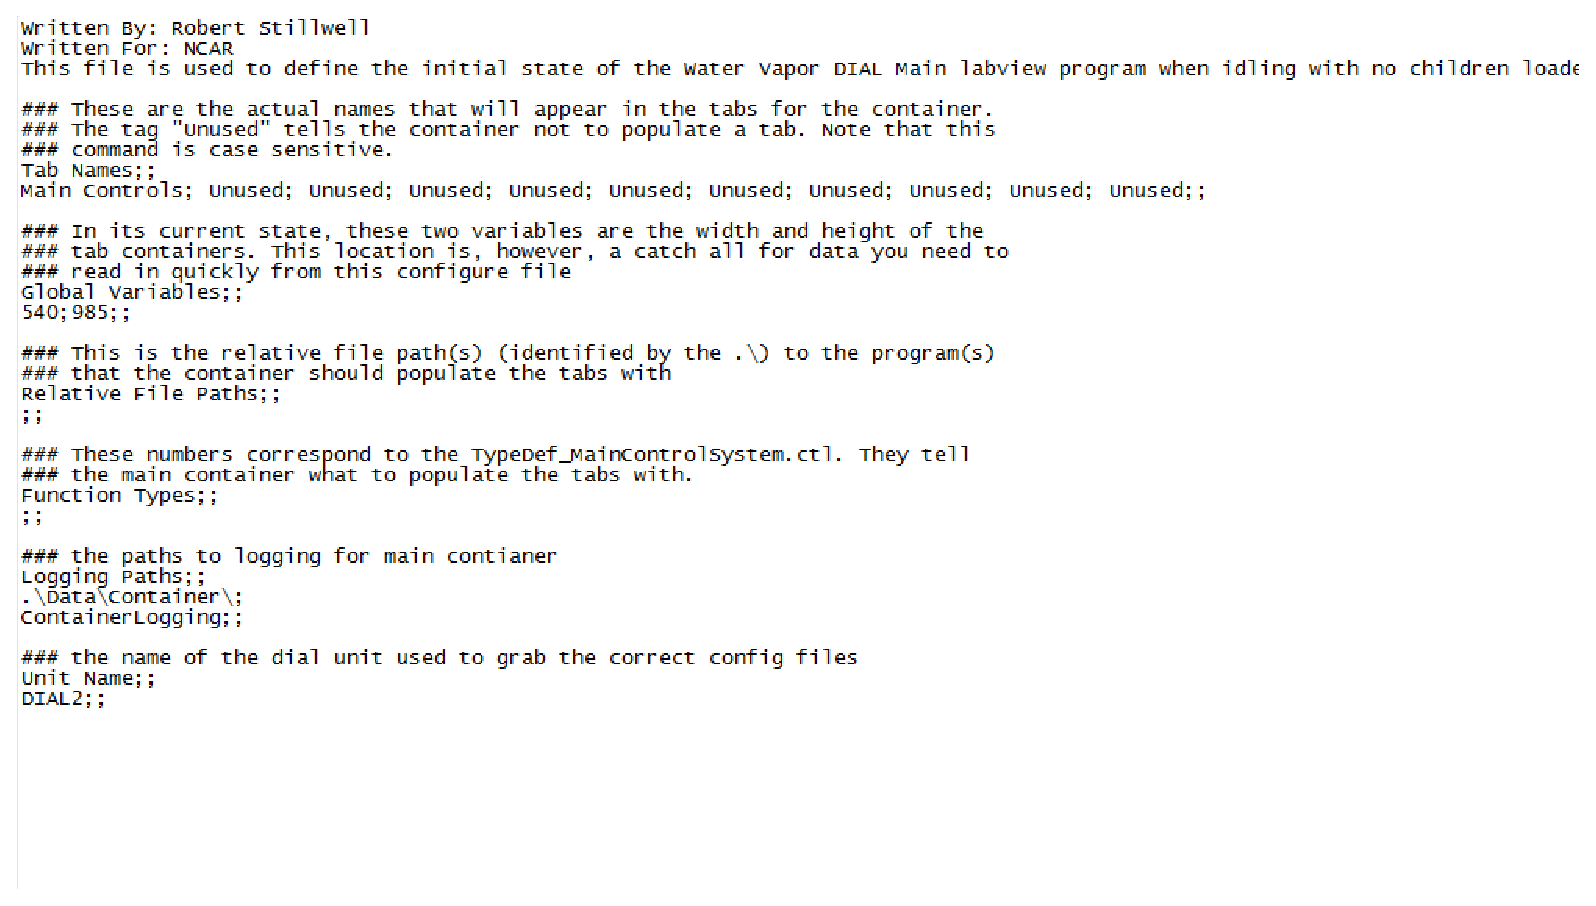
\includegraphics[height=3in]{Figures/ConfigureFileExample}
\caption{An example of the structure of a configure file. Variables are identified by a single name followed by two semi-colons. The next line has the required values delimitated by a single semi-colon with the end of line denoted by a double semi-colon.}\label{Fig:ConfigureFile}
\end{figure}

If a configure file has been edited and a revert to a default state is required, local changes to the configure file can be discarded and replaced with the defaults from the github repository. This is accomplished from the git bash terminal by navigating to the ConfigureFiles directory for the unit and running a command like - 

git checkout $ \langle $ConfigureFileToCheckoutFromGithub$ \rangle $  

If you want to replace the configure file in the github repo with a currently functioning configure file, then run these commands from the git bash after navigating to the ConfigureFiles directory for the unit - 

git add $ \langle $ConfigureFileToAddToGithub$ \rangle $ 

git commit -m ``comment describing the commit''

git push

This assumes that your local repo is up to date with the remote repo. Much, much more can be learned through a google search about Git/Github including branches, releases, etc... than i will be able to describe here. 
